\documentclass[11pt,letterpaper]{article}
\topmargin -.5truein
\textheight 9.0truein
\oddsidemargin 0truein
\evensidemargin 0truein
\textwidth 6.5truein
\setlength{\parskip}{5pt}
\setlength\parindent{0pt}
\usepackage[table]{xcolor}% http://ctan.org/pkg/xcolor
\usepackage{caption}
\usepackage{subcaption}
\usepackage[round]{natbib}
\usepackage{graphicx}
\usepackage{listings}
\usepackage{amsmath}
\usepackage{amssymb}
\usepackage{qtree}
\usepackage{algorithmic}
\usepackage{wrapfig}
\usepackage{tikz}
\usepackage{dsfont}
\usepackage{multirow}
\usepackage[all]{xy}
\usetikzlibrary{arrows,snakes,backgrounds,patterns,matrix,shapes,fit,calc,shadows,plotmarks}



\newcommand{\bs}{\textbackslash}
\renewcommand{\vec}[1]{\mathbf{#1}}

\newcommand{\ngramstart}{\ensuremath{\langle \textsc{s} \rangle}}
\newcommand{\ngramend}{\ensuremath{\langle \textsc{e} \rangle}}
\newcommand{\ngramunk}{\ensuremath{\langle unk \rangle}}

\newcommand{\wcurr}{\ensuremath{w_i}}
\newcommand{\tcurr}{\ensuremath{t_i}}
\newcommand{\tprev}{\ensuremath{t_{i-1}}}

\usepackage{hyperref}
\hypersetup{
    colorlinks,
    citecolor=black,
    filecolor=black,
    linkcolor=black,
    urlcolor=black
}

\title{NLP: Hidden Markov Models}
\author{Dan Garrette\\\small{dhg@cs.utexas.edu}}

\begin{document}
\maketitle



\section{Tagging}

\begin{itemize}
  \item Named entities
  \item Parts of speech
\end{itemize}




\section{Parts of Speech}

Tagsets

\begin{itemize}
  \item Google Universal Tagset, 12: Noun, Verb, Adjective, Adverb, Pronoun, Determiner, Adposition (prepositions and postpositions), Numerals, Conjunctions, Particles, Punctuation, Other
  \item Penn Treebank, 45.  Includes 4 categores of noun, 4 categories of pronoun, and 6 categories of verb.
  \item Brown Corpus, 87
\end{itemize}

Deciding what categories

\begin{itemize}
  \item Auxilliary verbs?  ``I \textit{had} gone''
  \item Numbers as adjectives? ``I saw 4 cars''
  \item Count vs. mass nouns?  ``some apple'' vs. ``two apples'', ``some snow'' vs. ``two snows''
\end{itemize}

Uses

\begin{itemize}
  \item Parsing: determiner and noun should connect first, then to verb
  \item Speech synthesis: OBject (noun) vs. obJECT (verb), CONtent (noun) vs. conTENT (adj)
\end{itemize}

Rule-based

\begin{itemize}
  \item ``if it ends in `-tion' '' $\rightarrow$ Noun
  \item ``if it ends in `-ize' '' $\rightarrow$ Verb
  \item ``if it starts with `re-' '' $\rightarrow$ Verb
  \item ``if it starts with a capital letter'' $\rightarrow$ Proper Noun
  \item ``if it's preceded by `the' '' $\rightarrow$ Noun
  \item ``if it's followed by \textit{'s} '' $\rightarrow$ Noun
  \item ``if it's preceded by an adjective'' $\rightarrow$ Noun
  \item Or just memorize a big list of words and tags?
    \begin{itemize}
      \item Ambiguity?
      \item Picking the most common tag for a word $\rightarrow$ 90\% accuracy (thought state-of-the-art is 97\%)
    \end{itemize}
\end{itemize}

Open vs. Closed

\begin{itemize}
  \item Open class tags: new words are frequently added
    \begin{itemize}
      \item noun, verb, adjective, adverb
      \item ``Twitter'', to ``tweet'', ``twitterish''
    \end{itemize}
  \item Closed class tags: new words are rarely added
    \begin{itemize}
      \item determiner, preposition, pronouns, ...
      \item Don't want to completely close off new words
      \item Maybe \textit{alongside} (preposition) wasn't seen in training, only test
      \item New domains: ``u'' as a pronoun
    \end{itemize}
\end{itemize}

Complexitites:

\begin{itemize}
  \item Ambiguity:
    \begin{itemize}
      \item ``buy a book'' (noun) vs. ``book a flight'' (verb)
      \item ``talk over the deal'' (particle) vs. ``talk over the phone'' (prep)
    \end{itemize}
  \item Phrasal verbs: ``turn down'', ``rule out''
    \begin{itemize}
      \item ``he went on for days''
      \item ``he went on a boat''
    \end{itemize}
\end{itemize}



\section{Hidden Markov Models}


\begin{figure}[h]
\centering
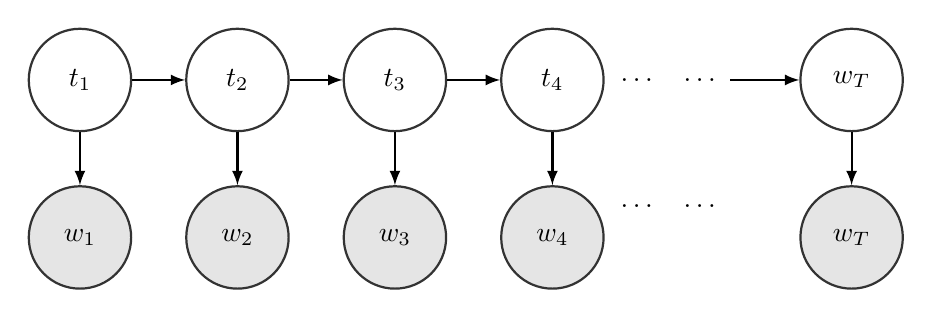
\begin{tikzpicture}
\tikzstyle{main}=[circle, minimum size = 13mm, thick, draw =black!80, node distance = 20mm]
\tikzstyle{obsv}=[main, fill = black!10]
\tikzstyle{hidden}=[node distance = 16mm]
\tikzstyle{connect}=[-latex, thick]
\tikzstyle{box}=[rectangle, draw=black!100]

  \node[main] (t1)                {$t_1$};
  \node[obsv] (w1) [below of =t1] {$w_1$};
  \node[main] (t2) [right of =t1] {$t_2$};
  \node[obsv] (w2) [below of =t2] {$w_2$};
  \node[main] (t3) [right of =t2] {$t_3$};
  \node[obsv] (w3) [below of =t3] {$w_3$};
  \node[main] (t4) [right of =t3] {$t_4$};
  \node[obsv] (w4) [below of =t4] {$w_4$};
  \node[hidden] (tI1) [right of =t4, xshift=-5mm] {$\dots$};
  \node[hidden] (wI1) [below of =tI1] {$\dots$};
  \node[hidden] (tI2) [right of =tI1, xshift=-8mm] {$\dots$};
  \node[hidden] (wI2) [below of =tI2] {$\dots$};
  \node[main] (tT) [right of=tI2, xshift=-1mm] {$w_T$};
  \node[obsv] (wT) [below of=tT] {$w_T$};

  \path (t1) edge [connect] (t2)
        (t2) edge [connect] (t3)
        (t3) edge [connect] (t4)
        (tI2) edge [connect] (tT)
        (t1) edge [connect] (w1)
        (t2) edge [connect] (w2)
        (t3) edge [connect] (w3)
        (t4) edge [connect] (w4)
        (tT) edge [connect] (wT);

\end{tikzpicture}
\caption{Second-order HMM showing conditional dependencies}
\end{figure} 

\begin{figure}[h]
\centering
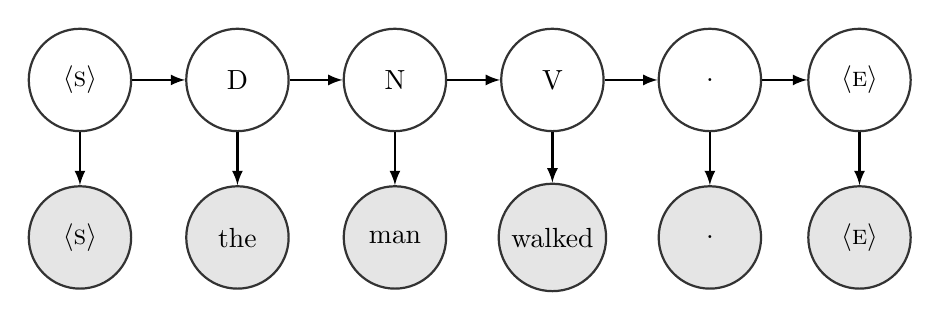
\begin{tikzpicture}
\tikzstyle{main}=[circle, minimum size = 13mm, thick, draw =black!80, node distance = 20mm]
\tikzstyle{obsv}=[main, fill = black!10]
\tikzstyle{hidden}=[node distance = 16mm]
\tikzstyle{connect}=[-latex, thick]
\tikzstyle{box}=[rectangle, draw=black!100]

  \node[main] (t1)                {\ngramstart};
  \node[obsv] (w1) [below of =t1] {\ngramstart};
  \node[main] (t2) [right of =t1] {D};
  \node[obsv] (w2) [below of =t2] {the};
  \node[main] (t3) [right of =t2] {N};
  \node[obsv] (w3) [below of =t3] {man};
  \node[main] (t4) [right of =t3] {V};
  \node[obsv] (w4) [below of =t4] {walked};
  \node[main] (t7) [right of =t4] {.};
  \node[obsv] (w7) [below of =t7] {.};
  \node[main] (tT) [right of =t7, xshift=-1mm] {\ngramend};
  \node[obsv] (wT) [below of =tT] {\ngramend};

  \path (t1) edge [connect] (t2)
        (t2) edge [connect] (t3)
        (t3) edge [connect] (t4)
        (t4) edge [connect] (t7)
        (t7) edge [connect] (tT)

        (t1) edge [connect] (w1)
        (t2) edge [connect] (w2)
        (t3) edge [connect] (w3)
        (t4) edge [connect] (w4)
        (t7) edge [connect] (w7)
        (tT) edge [connect] (wT);

\end{tikzpicture}
\caption{Second-order HMM for the sentence ``the man walks .''}
\end{figure} 



Similar to N-Gram models

\begin{itemize}
  \item Model the text as a \textit{sequence}
    \begin{itemize}
      \item Bad assumption, but less sparse
    \end{itemize}
  \item For ngrams, we modeled the probability of each word conditioned on the previous n-1 words.
  \item Here, we model each \textit{tag} conditioned on previous \textit{tags}
  \item Still uses Markov assumption: only look back a few tags
    \begin{itemize}
      \item Again, bad assumption, but less sparse
    \end{itemize}
  \item Note that we have to condition words on tags because otherwise 
\end{itemize}


~\\ \bs\bs~ Day 2 \\

Derivation

\begin{itemize}
  \item We want the most likely tag sequence for a sequence of words: \vspace{2mm} \\
        $~~~~~~~~~~p(\ngramstart~t_1~t_2~...~t_n~\ngramend \mid \ngramstart~w_1~w_2~...~w_n~\ngramend)$
        \vspace{2mm} \\ Remember that order matters!
  \item For simplicity, we'll write this as $t_1^n = \langle t_1, t_2, ..., t_n \rangle$
  \item So we want  \vspace{2mm} \\
  $~~~~~~~~~~~~~\hat{t}_1^n = \text{argmax}_{t_1^n}~p(\ngramstart~t_1~t_2~...~t_n~\ngramend \mid \ngramstart~w_1~w_2~...~w_n~\ngramend)$ \vspace{2mm} \\ but it's hard to estimate
  \item Like for ngrams, use Bayes rule: 
  \begin{align*}
  \hat{t}_1^n 
  &= \text{argmax}_{t_1^n}~\frac{p(\ngramstart~w_1~w_2~...~w_n~\ngramend \mid \ngramstart~t_1~t_2~...~t_n~\ngramend) \cdot p(\ngramstart~t_1~t_2~...~t_n~\ngramend}{p(\ngramstart~w_1~w_2~...~w_n~\ngramend)} \\
  & = \text{argmax}_{t_1^n}~p(\ngramstart~w_1~w_2~...~w_n~\ngramend \mid \ngramstart~t_1~t_2~...~t_n~\ngramend) \cdot p(\ngramstart~t_1~t_2~...~t_n~\ngramend)
\end{align*}

  \item Two major independence assumptions:
    \begin{itemize}
      \item Like ngrams, assume probability of a sequence is dependent only on recent past:
        \begin{align*}
          p(\ngramstart~t_1~t_2~...~t_n~\ngramend) 
                    &\approx p(t_1 \mid \ngramstart) \cdot 
                              p(t_2 \mid t_1) \cdot 
                              p(t_2 \mid t_2) \cdot 
                              ...  \cdot 
                              p(t_n \mid t_{n-1}) \cdot 
                              p(\ngramend \mid t_n) \\
                    &= \prod_{i=1}^n p(t_i \mid t_{i-1})
        \end{align*}
      \item Also assume word is only dependent on its tag: \vspace{2mm}
        \begin{align*}
          p(\ngramstart~w_1~w_2~...~w_n~\ngramend \mid \ngramstart~t_1~t_2~...~t_n~\ngramend) 
                    &\approx p(w_1 \mid t_1) \cdot 
                             p(w_2 \mid t_2) \cdot 
                             ...  \cdot 
                             p(w_n \mid t_n) \\
                    &= \prod_{i=1}^n p(w_i \mid t_i)
        \end{align*}
      \item Together: 
        \begin{align*}
        \hat{t}_1^n &= \text{argmax}_{t_1^n}~p(\ngramstart~t_1~t_2~...~t_n~\ngramend \mid \ngramstart~w_1~w_2~...~w_n~\ngramend) \\
                    &= \text{argmax}_{t_1^n}~p(\ngramstart~w_1~w_2~...~w_n~\ngramend \mid \ngramstart~t_1~t_2~...~t_n~\ngramend) &&\hspace{-7mm}\cdot p(\ngramstart~t_1~t_2~...~t_n~\ngramend) \\
                    &\approx \text{argmax}_{t_1^n}~\prod_{i=1}^n p(w_i \mid t_i) &&\hspace{-7mm}\cdot \prod_{i=1}^n p(t_i \mid t_{i-1}) \\
                    &= \text{argmax}_{t_1^n}~\prod_{i=1}^n p(w_i \mid t_i) \cdot p(t_i \mid t_{i-1})
        \end{align*}
    \end{itemize}
\end{itemize}


\section{Estimating Parameters: MLE}

Two probability distributions to estimate:

\begin{itemize}
  \item Transitions: probability of a tag, given previous tag, $p(t_i \mid t_{i-1})$
  \item Emissions: probability of a word, given its tag, $p(w_i \mid t_i)$
\end{itemize}

MLE

\begin{itemize}
  \item MLE estimation is just like before (na\"{i}ve Bayes, ngrams, ...): normalized counts
  \item Transitions: $p(t_i \mid t_{i-1}) = \frac{C(t_{i-1}~t_i)}{\sum_x C(t_{i-1}~x)} = \frac{C(t_{i-1}~t_i)}{C(t_{i-1})}$
  \item Emissions: $p(w_i \mid t_i) = \frac{C(t_i,w_i)}{\sum_x C(t_i,x)} = \frac{C(t_i,w_i)}{C(t_i)}$
\end{itemize}

Example dataset (punctuation excluded for simplicity!):
\vspace{-2mm}
\begin{verbatim}
    <S>|<S> the|D man|N walks|V the|D dog|N <E>|<E> 
    <S>|<S> the|D dog|N runs|V <E>|<E> 
    <S>|<S> the|D dog|N walks|V <E>|<E> 
    <S>|<S> the|D man|N walks|V <E>|<E> 
    <S>|<S> a|D man|N saw|V the|D dog|N <E>|<E> 
    <S>|<S> the|D cat|N walks|V <E>|<E> 
\end{verbatim}

Some probabilities:

\begin{itemize}
  \item $p(t_i=\text{V} \mid t_{i-1}=\text{N}) = \frac{C(\text{N V})}{\sum_x C(\text{N } x)} = \frac{6}{8} = 0.75$
  \item $p(t_i=\text{D} \mid t_{i-1}=\text{N}) = \frac{C(\text{N D})}{\sum_x C(\text{N } x)} = \frac{0}{8} = 0.0$
  \\
  \item $p(w_i=\text{dog} \mid t_i=\text{N}) = \frac{C(\text{N,dog})}{\sum_x C(\text{N},x)} = \frac{4}{8} = 0.50$
  \item $p(w_i=\text{the} \mid t_i=\text{N}) = \frac{C(\text{N,the})}{\sum_x C(\text{N},x)} = \frac{0}{8} = 0.0$
\end{itemize}


\section{Add-$\lambda$ Smoothing}

Again, just like before.

\begin{itemize}
  \item Transitions: $p(t_i \mid t_{i-1}) 
             = \frac{C(t_{i-1}~t_i)+\lambda}{\sum_x (C(t_{i-1}~x)+\lambda)} 
             = \frac{C(t_{i-1}~t_i)+\lambda}{(\sum_x C(t_{i-1}~x))+\lambda\cdot|T|} 
             = \frac{C(t_{i-1}~t_i)}{C(t_{i-1})}$
  \item Emissions: $p(w_i \mid t_i) 
             = \frac{C(t_i,w_i)+\lambda}{\sum_x (C(t_i,x)+\lambda)} 
             = \frac{C(t_i,w_i)+\lambda}{(\sum_x C(t_i,x))+\lambda\cdot|V|} 
             = \frac{C(t_i,w_i)}{C(t_i)}$
\end{itemize}

Some probabilities (with $\lambda=2$):

\begin{itemize}
  \item The Vocabulary $V$ is the set of all word types that might be associated with a tag \tcurr:   \vspace{2mm} \\
  $V = \{ a, cat, dog, man, runs, saw, the, walks \}$, ~~$|V|=8$
  \item The Tagset $T$ is the set of all possible tags that could follow a tag \tprev:   \vspace{2mm} \\
        $T = \{ D, N, V, \ngramend \}$, ~~$|T|=4$
  \\
  \item $p(t_i=\text{V} \mid t_{i-1}=\text{N}) 
     = \frac{C(\text{N V})+2}{\sum_{x \in T} (C(\text{N } x)+2)} 
     = \frac{C(\text{N V})+2}{(\sum_{x \in T} C(\text{N } x))+(2 \cdot 4)} 
     = \frac{6+2}{8+8} 
     = \frac{8}{16} = 0.50$
  \item $p(t_i=\text{D} \mid t_{i-1}=\text{N}) 
     = \frac{C(\text{N D})+2}{\sum_{x \in T} (C(\text{N } x)+2)} 
     = \frac{C(\text{N D})+2}{(\sum_{x \in T} C(\text{N } x))+(2 \cdot 4)} 
     = \frac{0+2}{8+8}
     = \frac{2}{16} = 0.125$
  \\
  \item $p(w_i=\text{dog} \mid t_i=\text{N}) 
     = \frac{C(\text{N,dog})}{\sum_{x \in V} (C(\text{N},x)+2)} 
     = \frac{C(\text{N,dog})}{(\sum_{x \in V} C(\text{N},x))+(2 \cdot 8)} 
     = \frac{4+2}{8+16}
     = 0.25$
  \item $p(w_i=\text{the} \mid t_i=\text{N}) 
     = \frac{C(\text{N,the})}{\sum_{x \in V} (C(\text{N},x)+2)} 
     = \frac{C(\text{N,the})}{(\sum_{x \in V} C(\text{N},x))+(2 \cdot 8)} 
     = \frac{0+2}{8+16} 
     = 0.08$
\end{itemize}

Differences:

\begin{itemize}
  \item Two distributions, two kinds of smoothing
  \item Can do add-$\lambda$ for both, but don't need to use same $\lambda$
  \item Can use totally different smoothing for each.
\end{itemize}


\section{One-Count Smoothing}

From Chen and Goodman (1996)

Idea: Smooth conditional distribution by interpolating the MLE with a unigram distribution where the degree of smoothing is proportional to the ``openness'' of a tag.
\begin{align*}
  p(\wcurr \mid \tcurr) &= \frac{C(\tcurr,\wcurr) + \alpha(\tcurr) \cdot p(\wcurr)}{C(\tcurr) + \alpha(\tcurr)}
  &&\text{where} ~~ \alpha(\tcurr) = | \wcurr: C(\tcurr,\wcurr) = 1 | \\
  p(\tcurr \mid \tprev) &= \frac{C(\tprev,\tcurr) + \lambda(\tprev) \cdot p(\tcurr)}{C(\tprev) + \lambda(\tprev)}
  &&\text{where} ~~ \lambda(\tprev) = | \tcurr: C(\tprev,\tcurr) = 1 |
\end{align*}

\begin{itemize}
  \item For emissions, if a tag \tcurr\ appears one time with a large number of word types, then we assume that it is very ``open'': there is a large number of words that it has only been seen with once, so the likelihood that it \textit{could have} been seen with some other word, even though it didn't \textit{happen} to be seen with it, is high.
  \item For transition, the reasoning is the same.  Instead of a tag being associated with a wide variety of words once, it's a wide variety of subsequent tags once.
\end{itemize}


\section{Decoding}

Tagging a sentence

\begin{itemize}
  \item $\text{argmax}_{t_1^n}~\prod_{i=1}^n p(w_i \mid t_i) \cdot p(t_i \mid t_{i-1})$
  \item For ``the dog walks .'', we have to check all combinations: \vspace{2mm} \\
        \ngramstart\ D D D D \ngramend  \vspace{2mm} \\
        \ngramstart\ N D D D \ngramend  \vspace{2mm} \\
        \ngramstart\ V D D D \ngramend  \vspace{2mm} \\
        \ngramstart\ . D D D \ngramend  \vspace{2mm} \\
        \ngramstart\ N N D D \ngramend  \vspace{2mm} \\
        \ngramstart\ N V D D \ngramend  \vspace{2mm} \\
        ...
  \item But this is insane.
\end{itemize}



~\\ \bs\bs~ Day 3 \\

Choosing a tag

\begin{itemize}
  \item Because of our independence assumptions, the probability of each tag is dependent only on its ``Markov blanket'': the previous tag, emitted word, and next tag.  
    \begin{align*} p(t_i \mid \ngramstart~w_1~w_2~...~w_n~\ngramend, \ngramstart~t_1~t_2~...~\mathbf{t_{i-1}~t_{i+1}}~...~t_n~\ngramend)
       &= p(t_i \mid t_{i-1}, w_i, t_{i+1}) \\
       &= p(t_i \mid t_{i-1}) \cdot p(w_i \mid t_i) \cdot p(t_{i+1} \mid t_i)
    \end{align*}
\end{itemize}

Tagging a sentence

\begin{itemize}
  \item We want to make global decisions about tags.
  \item Due to independence, global decisions are made in terms of local decisions
  \item Tagging ``forward'' through the sentence allows us to predict tags based on previous decisions.
  \item But we can't calculate picking a tag changes the probabilities of previous tags.
\end{itemize}

Dynamic Programming:

\begin{itemize}
  \item We need to check all possible tag combinations \textit{efficiently}
  \item We do this by making two passes through the sentence: one ``forward'' and one ``backward''
  \item The \textit{forward} pass: The Forward Algorithm
    \begin{itemize}
      \item Compute, for each potential tag value $k$ of \tcurr\ in the sentence, the likelihood of tagging $t_i=k$ given \textit{all possible ways of tagging the $i$-1 previous words}.
        \[
          p(t_i=k \mid w_{1:i}) = P(w_i \mid k) \cdot \sum_{k' \in T} P(k \mid k') \cdot p(t_{i-1}=k' \mid w_{1:i-1})
        \]
      \item Note that this is a \textit{recursive} definitio since the last probability is just the result of this same equation, but for the previous iteration.
      \item So $k$ is the potential tag for the current token $i$
      \item $k'$ is a potential tag for the previous token $i$-1.
      \item So this equation says that the likelihood of tagging \tcurr\ with some tag $k$ is the probability of emitting the word $w_i$ from $k$, times the sum of the probabilities of any possible tagging of the previous token $i$-1 with some tag $k'$ (given all of \textit{its} possible previous taggings) times the probability of transitioning from $k'$ to $k$.
      \item In terms of the \textbf{Markov blanket}, this covers the connections to the previous tag and the emitted word
    \end{itemize}
  \item The \textit{backward} pass: The Viterbi Algorithm
    \begin{itemize}
      \item Starting at the end of the sentence, use the \textit{forward} values (probability of assigning a tag $k$ to $t_i$ given all possible previous taggings), to figure out the most likely tag $k$ for $t_i$.
      \item Each tag selection is based on 
        \[
          P(t_i=k \mid t_{i+1}, w_{1:n}) = P(t_i=k \mid w_{1:i}) \cdot P(t_{i+1} \mid t_i=k)
        \]
      \item So:
        \[
          \hat{t}_i = \text{argmax}_k~P(t_i=k \mid w_{1:i}) \cdot P(t_{i+1} \mid t_i=k)
        \]
      \item In terms of the \textbf{Markov blanket}, this adds in the connection to the next tag (since it has now been decided) to the forward probability which is made up of connections to the previous tag and the emitted word
    \end{itemize}
\end{itemize}


\textbf{Example:} Tag the sentence: ``the dog walks''

\begin{figure}[h]
\centering
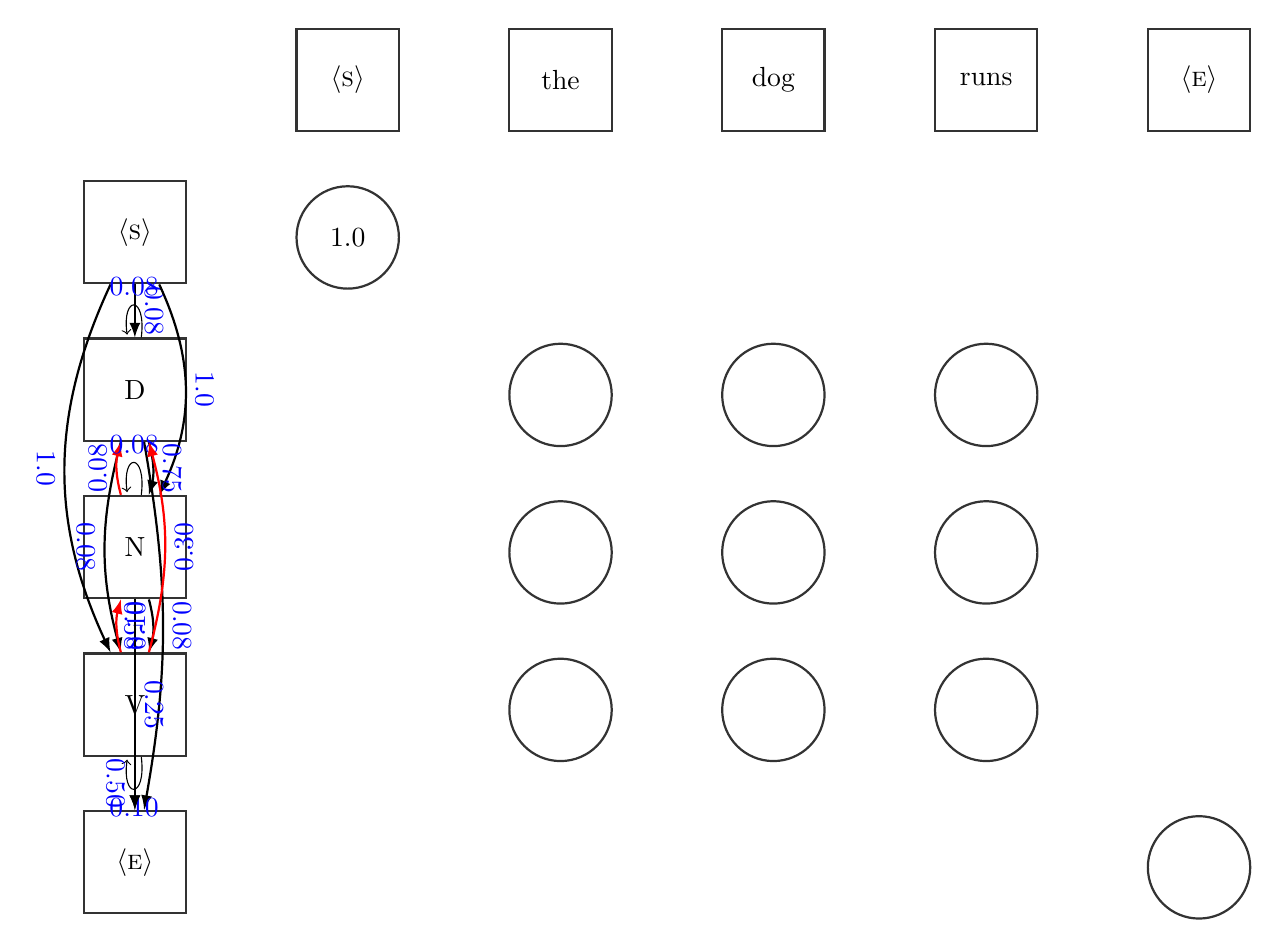
\begin{tikzpicture}
\tikzstyle{main}=[circle, thick, draw =black!80, node distance = 20mm, minimum size = 13mm]
\tikzstyle{rect}=[main, rectangle]
\tikzstyle{obsv}=[main, fill = black!10]
\tikzstyle{hidden}=[main, draw=white]
\tikzstyle{connect}=[-latex, thick]
\tikzstyle{box}=[rectangle, draw=black!100]

  
  \node[rect] (start) []                {\ngramstart};
  \node[rect] (D)     [below of =start] {D};
  \node[rect] (N)     [below of =D]     {N};
  \node[rect] (V)     [below of =N]     {V};
  \node[rect] (end)   [below of =V]     {\ngramend};

  \node[rect] (starttok) [right of =start,    xshift=20, yshift=55]   {\ngramstart};
  \node[rect] (the)      [right of =starttok, xshift=20]              {the};
  \node[rect] (dog)      [right of =the,      xshift=20]              {dog};
  \node[rect] (runs)     [right of =dog,      xshift=20]              {runs};
  \node[rect] (endtok)   [right of =runs,     xshift=20]              {\ngramend};

  \node[main] (startstart)  [below of =starttok]  {1.0};

  \node[hidden] (startthe)  [below of =the]       {};
  \node[main] (Dthe)        [below of =startthe]  {};
  \node[main] (Nthe)        [below of =Dthe]      {};
  \node[main] (Vthe)        [below of =Nthe]      {};
  \node[hidden] (endthe)    [below of =Vthe]      {};

  \node[hidden] (startdog)  [below of =dog]       {};
  \node[main] (Ddog)        [below of =startdog]  {};
  \node[main] (Ndog)        [below of =Ddog]      {};
  \node[main] (Vdog)        [below of =Ndog]      {};
  \node[hidden] (enddog)    [below of =Vdog]      {};

  \node[hidden] (startruns) [below of =runs]      {};
  \node[main] (Druns)       [below of =startruns] {};
  \node[main] (Nruns)       [below of =Druns]     {};
  \node[main] (Vruns)       [below of =Nruns]     {};
  \node[hidden] (endruns)   [below of =Vruns]     {};

  \node[hidden] (startend)  [below of =endtok]    {};
  \node[hidden] (Dend)      [below of =startend]  {};
  \node[hidden] (Nend)      [below of =Dend]      {};
  \node[hidden] (Vend)      [below of =Nend]      {};
  \node[main]   (endend)    [below of =Vend]      {};


  \path (start) edge [connect] node [pos=0.5, above, blue, sloped] {0.08} (D);
  \path (start) edge [connect, bend left=25] node [pos=0.5, above, blue, sloped] {1.0} (N);
  \path (start) edge [connect, bend right=25] node [pos=0.5, below, blue, sloped] {1.0} (V);
  
  \path (D) edge [in=98,out=83,loop] node [pos=0.5, above, blue, sloped] {0.08} (D);
  \path (D) edge [connect, bend left=15] node [pos=0.5, above, blue, sloped] {0.75} (N);
  \path (D) edge [connect, bend right=15] node [pos=0.5, below, blue, sloped] {0.08} (V);
  \path (D) edge [connect, bend left=10] node [pos=0.5, above, blue, sloped] {0.08} (end);

  \path (N) edge [connect, bend left=15, red] node [pos=0.5, above, blue, sloped] {0.08} (D);
  \path (N) edge [in=98,out=83,loop] node [pos=0.5, above, blue, sloped] {0.08} (N);
  \path (N) edge [connect, bend left=15] node [pos=0.5, below, blue, sloped] {0.58} (V);
  \path (N) edge [connect] node [pos=0.5, above, blue, sloped] {0.25} (end);

  \path (V) edge [connect, bend right=15, red] node [pos=0.5, below, blue, sloped] {0.30} (D);
  \path (V) edge [connect, bend left=15, red] node [pos=0.5, below, blue, sloped] {0.10} (N);
  \path (V) edge [in=-98,out=-83,loop] node [pos=0.5, below, blue, sloped] {0.10} (V);
  \path (V) edge [connect] node [pos=0.5, below, blue, sloped] {0.50} (end);
  

\end{tikzpicture}
\caption{}
\end{figure} 



\begin{figure}[h]
\centering
\begin{tikzpicture}
\tikzstyle{main}=[circle, thick, draw =black!80, node distance = 20mm, minimum size = 13mm]
\tikzstyle{rect}=[main, rectangle]
\tikzstyle{obsv}=[main, fill = black!10]
\tikzstyle{hidden}=[main, draw=white]
\tikzstyle{connect}=[-latex, thick]
\tikzstyle{box}=[rectangle, draw=black!100]

  
  \node[rect] (start) []                {\ngramstart};
  \node[rect] (D)     [below of =start] {D};
  \node[rect] (N)     [below of =D]     {N};
  \node[rect] (V)     [below of =N]     {V};
  \node[rect] (end)   [below of =V]     {\ngramend};

  \node[rect] (starttok) [right of =start,    xshift=20, yshift=55]   {\ngramstart};
  \node[rect] (the)      [right of =starttok, xshift=20]              {the};
  \node[rect] (dog)      [right of =the,      xshift=20]              {dog};
  \node[rect] (runs)     [right of =dog,      xshift=20]              {runs};
  \node[rect] (endtok)   [right of =runs,     xshift=20]              {\ngramend};

  \node[main] (startstart)  [below of =starttok]  {1.0};

  \node[hidden] (startthe)  [below of =the]       {};
  \node[draw, draw=white] at ([shift={(85:0.95)}]Dthe) {\color{red}0.47};
  \node[main] (Dthe)        [below of =startthe]  {0.37};
  \node[draw, draw=white] at ([shift={(85:0.95)}]Nthe) {\color{red}0.06};
  \node[main] (Nthe)        [below of =Dthe]      {0.007};
  \node[draw, draw=white] at ([shift={(85:0.95)}]Vthe) {\color{red}0.07};
  \node[main] (Vthe)        [below of =Nthe]      {0.008};
  \node[hidden] (endthe)    [below of =Vthe]      {};

  \node[hidden] (startdog)  [below of =dog]       {};
  \node[main] (Ddog)        [below of =startdog]  {};
  \node[main] (Ndog)        [below of =Ddog]      {};
  \node[main] (Vdog)        [below of =Ndog]      {};
  \node[hidden] (enddog)    [below of =Vdog]      {};

  \node[hidden] (startruns) [below of =runs]      {};
  \node[main] (Druns)       [below of =startruns] {};
  \node[main] (Nruns)       [below of =Druns]     {};
  \node[main] (Vruns)       [below of =Nruns]     {};
  \node[hidden] (endruns)   [below of =Vruns]     {};

  \node[hidden] (startend)  [below of =endtok]    {};
  \node[hidden] (Dend)      [below of =startend]  {};
  \node[hidden] (Nend)      [below of =Dend]      {};
  \node[hidden] (Vend)      [below of =Nend]      {};
  \node[main]   (endend)    [below of =Vend]      {};


  
  \path (startstart) edge [connect] node [pos=0.5, above, blue, sloped] {0.78} (Dthe);
  \path (startstart) edge [connect] node [pos=0.5, above, blue, sloped] {0.11} (Nthe);
  \path (startstart) edge [connect] node [pos=0.5, above, blue, sloped] {0.11} (Vthe);
  

\end{tikzpicture}
\caption{}
\end{figure} 





\begin{figure}[h]
\centering
\begin{tikzpicture}
\tikzstyle{main}=[circle, thick, draw =black!80, node distance = 20mm, minimum size = 13mm]
\tikzstyle{rect}=[main, rectangle]
\tikzstyle{obsv}=[main, fill = black!10]
\tikzstyle{hidden}=[main, draw=white]
\tikzstyle{connect}=[-latex, thick]
\tikzstyle{box}=[rectangle, draw=black!100]

  
  \node[rect] (start) []                {\ngramstart};
  \node[rect] (D)     [below of =start] {D};
  \node[rect] (N)     [below of =D]     {N};
  \node[rect] (V)     [below of =N]     {V};
  \node[rect] (end)   [below of =V]     {\ngramend};

  \node[rect] (starttok) [right of =start,    xshift=20, yshift=55]   {\ngramstart};
  \node[rect] (the)      [right of =starttok, xshift=20]              {the};
  \node[rect] (dog)      [right of =the,      xshift=20]              {dog};
  \node[rect] (runs)     [right of =dog,      xshift=20]              {runs};
  \node[rect] (endtok)   [right of =runs,     xshift=20]              {\ngramend};

  \node[main] (startstart)  [below of =starttok]  {1.0};

  \node[hidden] (startthe)  [below of =the]       {};
  \node[main] (Dthe)        [below of =startthe]  {0.37};
  \node[main] (Nthe)        [below of =Dthe]      {0.007};
  \node[main] (Vthe)        [below of =Nthe]      {0.008};
  \node[hidden] (endthe)    [below of =Vthe]      {};

  \node[hidden] (startdog)  [below of =dog]       {};
  \node[draw, draw=white] at ([shift={(85:0.95)}]Ddog) {\color{red}0.06};
  \node[main] (Ddog)        [below of =startdog]  {0.002};
  \node[draw, draw=white] at ([shift={(85:0.95)}]Ndog) {\color{red}0.29};
  \node[main] (Ndog)        [below of =Ddog]      {};
  \node[draw, draw=white] at ([shift={(85:0.95)}]Vdog) {\color{red}0.07};
  \node[main] (Vdog)        [below of =Ndog]      {};
  \node[hidden] (enddog)    [below of =Vdog]      {};

  \node[hidden] (startruns) [below of =runs]      {};
  \node[main] (Druns)       [below of =startruns] {};
  \node[main] (Nruns)       [below of =Druns]     {};
  \node[main] (Vruns)       [below of =Nruns]     {};
  \node[hidden] (endruns)   [below of =Vruns]     {};

  \node[hidden] (startend)  [below of =endtok]    {};
  \node[hidden] (Dend)      [below of =startend]  {};
  \node[hidden] (Nend)      [below of =Dend]      {};
  \node[hidden] (Vend)      [below of =Nend]      {};
  \node[main]   (endend)    [below of =Vend]      {};


  
  \path (Dthe) edge [connect] node [pos=0.5, above, blue, sloped] {0.08} (Ddog);
  \path (Nthe) edge [connect] node [pos=0.5, above, blue, sloped] {0.08} (Ddog);
  \path (Vthe) edge [connect] node [pos=0.5, above, blue, sloped] {0.30} (Ddog);
  

\end{tikzpicture}
\caption{}
\end{figure} 





\begin{figure}[h]
\centering
\begin{tikzpicture}
\tikzstyle{main}=[circle, thick, draw =black!80, node distance = 20mm, minimum size = 13mm]
\tikzstyle{rect}=[main, rectangle]
\tikzstyle{obsv}=[main, fill = black!10]
\tikzstyle{hidden}=[main, draw=white]
\tikzstyle{connect}=[-latex, thick]
\tikzstyle{box}=[rectangle, draw=black!100]

  
  \node[rect] (start) []                {\ngramstart};
  \node[rect] (D)     [below of =start] {D};
  \node[rect] (N)     [below of =D]     {N};
  \node[rect] (V)     [below of =N]     {V};
  \node[rect] (end)   [below of =V]     {\ngramend};

  \node[rect] (starttok) [right of =start,    xshift=20, yshift=55]   {\ngramstart};
  \node[rect] (the)      [right of =starttok, xshift=20]              {the};
  \node[rect] (dog)      [right of =the,      xshift=20]              {dog};
  \node[rect] (runs)     [right of =dog,      xshift=20]              {runs};
  \node[rect] (endtok)   [right of =runs,     xshift=20]              {\ngramend};

  \node[main] (startstart)  [below of =starttok]  {1.0};

  \node[hidden] (startthe)  [below of =the]       {};
  \node[main] (Dthe)        [below of =startthe]  {0.37};
  \node[main] (Nthe)        [below of =Dthe]      {0.007};
  \node[main] (Vthe)        [below of =Nthe]      {0.008};
  \node[hidden] (endthe)    [below of =Vthe]      {};

  \node[hidden] (startdog)  [below of =dog]       {};
  \node[draw, draw=white] at ([shift={(85:0.95)}]Ddog) {\color{red}0.06};
  \node[main] (Ddog)        [below of =startdog]  {0.002};
  \node[draw, draw=white] at ([shift={(85:0.95)}]Ndog) {\color{red}0.29};
  \node[main] (Ndog)        [below of =Ddog]      {0.08};
  \node[draw, draw=white] at ([shift={(85:0.95)}]Vdog) {\color{red}0.07};
  \node[main] (Vdog)        [below of =Ndog]      {};
  \node[hidden] (enddog)    [below of =Vdog]      {};

  \node[hidden] (startruns) [below of =runs]      {};
  \node[main] (Druns)       [below of =startruns] {};
  \node[main] (Nruns)       [below of =Druns]     {};
  \node[main] (Vruns)       [below of =Nruns]     {};
  \node[hidden] (endruns)   [below of =Vruns]     {};

  \node[hidden] (startend)  [below of =endtok]    {};
  \node[hidden] (Dend)      [below of =startend]  {};
  \node[hidden] (Nend)      [below of =Dend]      {};
  \node[hidden] (Vend)      [below of =Nend]      {};
  \node[main]   (endend)    [below of =Vend]      {};


  
  \path (Dthe) edge [connect] node [pos=0.5, above, blue, sloped] {0.75} (Ndog);
  \path (Nthe) edge [connect] node [pos=0.5, above, blue, sloped] {0.08} (Ndog);
  \path (Vthe) edge [connect] node [pos=0.5, above, blue, sloped] {0.10} (Ndog);
  

\end{tikzpicture}
\caption{}
\end{figure} 





\begin{figure}[h]
\centering
\begin{tikzpicture}
\tikzstyle{main}=[circle, thick, draw =black!80, node distance = 20mm, minimum size = 13mm]
\tikzstyle{rect}=[main, rectangle]
\tikzstyle{obsv}=[main, fill = black!10]
\tikzstyle{hidden}=[main, draw=white]
\tikzstyle{connect}=[-latex, thick]
\tikzstyle{box}=[rectangle, draw=black!100]

  
  \node[rect] (start) []                {\ngramstart};
  \node[rect] (D)     [below of =start] {D};
  \node[rect] (N)     [below of =D]     {N};
  \node[rect] (V)     [below of =N]     {V};
  \node[rect] (end)   [below of =V]     {\ngramend};

  \node[rect] (starttok) [right of =start,    xshift=20, yshift=55]   {\ngramstart};
  \node[rect] (the)      [right of =starttok, xshift=20]              {the};
  \node[rect] (dog)      [right of =the,      xshift=20]              {dog};
  \node[rect] (runs)     [right of =dog,      xshift=20]              {runs};
  \node[rect] (endtok)   [right of =runs,     xshift=20]              {\ngramend};

  \node[main] (startstart)  [below of =starttok]  {1.0};

  \node[hidden] (startthe)  [below of =the]       {};
  \node[main] (Dthe)        [below of =startthe]  {0.37};
  \node[main] (Nthe)        [below of =Dthe]      {0.007};
  \node[main] (Vthe)        [below of =Nthe]      {0.008};
  \node[hidden] (endthe)    [below of =Vthe]      {};

  \node[hidden] (startdog)  [below of =dog]       {};
  \node[draw, draw=white] at ([shift={(85:0.95)}]Ddog) {\color{red}0.06};
  \node[main] (Ddog)        [below of =startdog]  {0.002};
  \node[draw, draw=white] at ([shift={(85:0.95)}]Ndog) {\color{red}0.29};
  \node[main] (Ndog)        [below of =Ddog]      {0.08};
  \node[draw, draw=white] at ([shift={(85:0.95)}]Vdog) {\color{red}0.07};
  \node[main] (Vdog)        [below of =Ndog]      {0.002};
  \node[hidden] (enddog)    [below of =Vdog]      {};

  \node[hidden] (startruns) [below of =runs]      {};
  \node[main] (Druns)       [below of =startruns] {};
  \node[main] (Nruns)       [below of =Druns]     {};
  \node[main] (Vruns)       [below of =Nruns]     {};
  \node[hidden] (endruns)   [below of =Vruns]     {};

  \node[hidden] (startend)  [below of =endtok]    {};
  \node[hidden] (Dend)      [below of =startend]  {};
  \node[hidden] (Nend)      [below of =Dend]      {};
  \node[hidden] (Vend)      [below of =Nend]      {};
  \node[main]   (endend)    [below of =Vend]      {};


  
  \path (Dthe) edge [connect] node [pos=0.5, above, blue, sloped] {0.08} (Vdog);
  \path (Nthe) edge [connect] node [pos=0.5, above, blue, sloped] {0.58} (Vdog);
  \path (Vthe) edge [connect] node [pos=0.5, above, blue, sloped] {0.10} (Vdog);
  

\end{tikzpicture}
\caption{}
\end{figure} 






\begin{figure}[h]
\centering
\begin{tikzpicture}
\tikzstyle{main}=[circle, thick, draw =black!80, node distance = 20mm, minimum size = 13mm]
\tikzstyle{rect}=[main, rectangle]
\tikzstyle{obsv}=[main, fill = black!10]
\tikzstyle{hidden}=[main, draw=white]
\tikzstyle{connect}=[-latex, thick]
\tikzstyle{box}=[rectangle, draw=black!100]

  
  \node[rect] (start) []                {\ngramstart};
  \node[rect] (D)     [below of =start] {D};
  \node[rect] (N)     [below of =D]     {N};
  \node[rect] (V)     [below of =N]     {V};
  \node[rect] (end)   [below of =V]     {\ngramend};

  \node[rect] (starttok) [right of =start,    xshift=20, yshift=55]   {\ngramstart};
  \node[rect] (the)      [right of =starttok, xshift=20]              {the};
  \node[rect] (dog)      [right of =the,      xshift=20]              {dog};
  \node[rect] (runs)     [right of =dog,      xshift=20]              {runs};
  \node[rect] (endtok)   [right of =runs,     xshift=20]              {\ngramend};

  \node[main] (startstart)  [below of =starttok]  {1.0};

  \node[hidden] (startthe)  [below of =the]       {};
  \node[main] (Dthe)        [below of =startthe]  {0.37};
  \node[main] (Nthe)        [below of =Dthe]      {0.007};
  \node[main] (Vthe)        [below of =Nthe]      {0.008};
  \node[hidden] (endthe)    [below of =Vthe]      {};

  \node[hidden] (startdog)  [below of =dog]       {};
  \node[main] (Ddog)        [below of =startdog]  {0.002};
  \node[main] (Ndog)        [below of =Ddog]      {0.08};
  \node[main] (Vdog)        [below of =Ndog]      {0.002};
  \node[hidden] (enddog)    [below of =Vdog]      {};

  \node[hidden] (startruns) [below of =runs]      {};
  \node[draw, draw=white] at ([shift={(85:0.95)}]Druns) {\color{red}0.06};
  \node[main] (Druns)       [below of =startruns] {0.0004};
  \node[draw, draw=white] at ([shift={(85:0.95)}]Nruns) {\color{red}0.06};
  \node[main] (Nruns)       [below of =Druns]     {};
  \node[draw, draw=white] at ([shift={(85:0.95)}]Vruns) {\color{red}0.13};
  \node[main] (Vruns)       [below of =Nruns]     {};
  \node[hidden] (endruns)   [below of =Vruns]     {};

  \node[hidden] (startend)  [below of =endtok]    {};
  \node[hidden] (Dend)      [below of =startend]  {};
  \node[hidden] (Nend)      [below of =Dend]      {};
  \node[hidden] (Vend)      [below of =Nend]      {};
  \node[main]   (endend)    [below of =Vend]      {};


  
  \path (Ddog) edge [connect] node [pos=0.5, above, blue, sloped] {0.08} (Druns);
  \path (Ndog) edge [connect] node [pos=0.5, above, blue, sloped] {0.08} (Druns);
  \path (Vdog) edge [connect] node [pos=0.5, above, blue, sloped] {0.30} (Druns);
  

\end{tikzpicture}
\caption{}
\end{figure} 





\begin{figure}[h]
\centering
\begin{tikzpicture}
\tikzstyle{main}=[circle, thick, draw =black!80, node distance = 20mm, minimum size = 13mm]
\tikzstyle{rect}=[main, rectangle]
\tikzstyle{obsv}=[main, fill = black!10]
\tikzstyle{hidden}=[main, draw=white]
\tikzstyle{connect}=[-latex, thick]
\tikzstyle{box}=[rectangle, draw=black!100]

  
  \node[rect] (start) []                {\ngramstart};
  \node[rect] (D)     [below of =start] {D};
  \node[rect] (N)     [below of =D]     {N};
  \node[rect] (V)     [below of =N]     {V};
  \node[rect] (end)   [below of =V]     {\ngramend};

  \node[rect] (starttok) [right of =start,    xshift=20, yshift=55]   {\ngramstart};
  \node[rect] (the)      [right of =starttok, xshift=20]              {the};
  \node[rect] (dog)      [right of =the,      xshift=20]              {dog};
  \node[rect] (runs)     [right of =dog,      xshift=20]              {runs};
  \node[rect] (endtok)   [right of =runs,     xshift=20]              {\ngramend};

  \node[main] (startstart)  [below of =starttok]  {1.0};

  \node[hidden] (startthe)  [below of =the]       {};
  \node[main] (Dthe)        [below of =startthe]  {0.37};
  \node[main] (Nthe)        [below of =Dthe]      {0.007};
  \node[main] (Vthe)        [below of =Nthe]      {0.008};
  \node[hidden] (endthe)    [below of =Vthe]      {};

  \node[hidden] (startdog)  [below of =dog]       {};
  \node[main] (Ddog)        [below of =startdog]  {0.002};
  \node[main] (Ndog)        [below of =Ddog]      {0.08};
  \node[main] (Vdog)        [below of =Ndog]      {0.002};
  \node[hidden] (enddog)    [below of =Vdog]      {};

  \node[hidden] (startruns) [below of =runs]      {};
  \node[draw, draw=white] at ([shift={(85:0.95)}]Druns) {\color{red}0.06};
  \node[main] (Druns)       [below of =startruns] {0.0004};
  \node[draw, draw=white] at ([shift={(85:0.95)}]Nruns) {\color{red}0.06};
  \node[main] (Nruns)       [below of =Druns]     {0.0005};
  \node[draw, draw=white] at ([shift={(85:0.95)}]Vruns) {\color{red}0.13};
  \node[main] (Vruns)       [below of =Nruns]     {};
  \node[hidden] (endruns)   [below of =Vruns]     {};

  \node[hidden] (startend)  [below of =endtok]    {};
  \node[hidden] (Dend)      [below of =startend]  {};
  \node[hidden] (Nend)      [below of =Dend]      {};
  \node[hidden] (Vend)      [below of =Nend]      {};
  \node[main]   (endend)    [below of =Vend]      {};


  
  \path (Ddog) edge [connect] node [pos=0.5, above, blue, sloped] {0.75} (Nruns);
  \path (Ndog) edge [connect] node [pos=0.5, above, blue, sloped] {0.08} (Nruns);
  \path (Vdog) edge [connect] node [pos=0.5, above, blue, sloped] {0.07} (Nruns);
  

\end{tikzpicture}
\caption{}
\end{figure} 




\begin{figure}[h]
\centering
\begin{tikzpicture}
\tikzstyle{main}=[circle, thick, draw =black!80, node distance = 20mm, minimum size = 13mm]
\tikzstyle{rect}=[main, rectangle]
\tikzstyle{obsv}=[main, fill = black!10]
\tikzstyle{hidden}=[main, draw=white]
\tikzstyle{connect}=[-latex, thick]
\tikzstyle{box}=[rectangle, draw=black!100]

  
  \node[rect] (start) []                {\ngramstart};
  \node[rect] (D)     [below of =start] {D};
  \node[rect] (N)     [below of =D]     {N};
  \node[rect] (V)     [below of =N]     {V};
  \node[rect] (end)   [below of =V]     {\ngramend};

  \node[rect] (starttok) [right of =start,    xshift=20, yshift=55]   {\ngramstart};
  \node[rect] (the)      [right of =starttok, xshift=20]              {the};
  \node[rect] (dog)      [right of =the,      xshift=20]              {dog};
  \node[rect] (runs)     [right of =dog,      xshift=20]              {runs};
  \node[rect] (endtok)   [right of =runs,     xshift=20]              {\ngramend};

  \node[main] (startstart)  [below of =starttok]  {1.0};

  \node[hidden] (startthe)  [below of =the]       {};
  \node[main] (Dthe)        [below of =startthe]  {0.37};
  \node[main] (Nthe)        [below of =Dthe]      {0.007};
  \node[main] (Vthe)        [below of =Nthe]      {0.008};
  \node[hidden] (endthe)    [below of =Vthe]      {};

  \node[hidden] (startdog)  [below of =dog]       {};
  \node[main] (Ddog)        [below of =startdog]  {0.002};
  \node[main] (Ndog)        [below of =Ddog]      {0.08};
  \node[main] (Vdog)        [below of =Ndog]      {0.002};
  \node[hidden] (enddog)    [below of =Vdog]      {};

  \node[hidden] (startruns) [below of =runs]      {};
  \node[draw, draw=white] at ([shift={(85:0.95)}]Druns) {\color{red}0.06};
  \node[main] (Druns)       [below of =startruns] {0.0004};
  \node[draw, draw=white] at ([shift={(85:0.95)}]Nruns) {\color{red}0.06};
  \node[main] (Nruns)       [below of =Druns]     {0.0005};
  \node[draw, draw=white] at ([shift={(85:0.95)}]Vruns) {\color{red}0.13};
  \node[main] (Vruns)       [below of =Nruns]     {0.006};
  \node[hidden] (endruns)   [below of =Vruns]     {};

  \node[hidden] (startend)  [below of =endtok]    {};
  \node[hidden] (Dend)      [below of =startend]  {};
  \node[hidden] (Nend)      [below of =Dend]      {};
  \node[hidden] (Vend)      [below of =Nend]      {};
  \node[main]   (endend)    [below of =Vend]      {};


  
  \path (Ddog) edge [connect] node [pos=0.5, above, blue, sloped] {0.08} (Vruns);
  \path (Ndog) edge [connect] node [pos=0.5, above, blue, sloped] {0.58} (Vruns);
  \path (Vdog) edge [connect] node [pos=0.5, above, blue, sloped] {0.10} (Vruns);
  

\end{tikzpicture}
\caption{}
\end{figure} 





\begin{figure}[h]
\centering
\begin{tikzpicture}
\tikzstyle{main}=[circle, thick, draw =black!80, node distance = 20mm, minimum size = 13mm]
\tikzstyle{rect}=[main, rectangle]
\tikzstyle{obsv}=[main, fill = black!10]
\tikzstyle{hidden}=[main, draw=white]
\tikzstyle{connect}=[-latex, thick]
\tikzstyle{box}=[rectangle, draw=black!100]

  
  \node[rect] (start) []                {\ngramstart};
  \node[rect] (D)     [below of =start] {D};
  \node[rect] (N)     [below of =D]     {N};
  \node[rect] (V)     [below of =N]     {V};
  \node[rect] (end)   [below of =V]     {\ngramend};

  \node[rect] (starttok) [right of =start,    xshift=20, yshift=55]   {\ngramstart};
  \node[rect] (the)      [right of =starttok, xshift=20]              {the};
  \node[rect] (dog)      [right of =the,      xshift=20]              {dog};
  \node[rect] (runs)     [right of =dog,      xshift=20]              {runs};
  \node[rect] (endtok)   [right of =runs,     xshift=20]              {\ngramend};

  \node[main] (startstart)  [below of =starttok]  {1.0};

  \node[hidden] (startthe)  [below of =the]       {};
  \node[main] (Dthe)        [below of =startthe]  {0.37};
  \node[main] (Nthe)        [below of =Dthe]      {0.007};
  \node[main] (Vthe)        [below of =Nthe]      {0.008};
  \node[hidden] (endthe)    [below of =Vthe]      {};

  \node[hidden] (startdog)  [below of =dog]       {};
  \node[main] (Ddog)        [below of =startdog]  {0.002};
  \node[main] (Ndog)        [below of =Ddog]      {0.08};
  \node[main] (Vdog)        [below of =Ndog]      {0.002};
  \node[hidden] (enddog)    [below of =Vdog]      {};

  \node[hidden] (startruns) [below of =runs]      {};
  \node[draw, draw=white] at ([shift={(75:-0.95)}]Druns) {\color{black!60!green}0.00003};
  \node[main] (Druns)       [below of =startruns] {0.0004};
  \node[draw, draw=white] at ([shift={(75:-0.95)}]Nruns) {\color{black!60!green}0.0001};
  \node[main] (Nruns)       [below of =Druns]     {0.0005};
  \node[draw, fill=white!50!green] at ([shift={(75:-0.95)}]Vruns) {\color{black!60!green}0.003};
  \node[main, fill=white!50!green] (Vruns)       [below of =Nruns]     {0.006};
  \node[hidden] (endruns)   [below of =Vruns]     {};

  \node[hidden] (startend)  [below of =endtok]    {};
  \node[hidden] (Dend)      [below of =startend]  {};
  \node[hidden] (Nend)      [below of =Dend]      {};
  \node[hidden] (Vend)      [below of =Nend]      {};
  \node[main]   (endend)    [below of =Vend]      {};


  
  \path (Druns) edge [connect] node [pos=0.35, above, blue, sloped] {0.08} (endend);
  \path (Nruns) edge [connect] node [pos=0.25, above, blue, sloped] {0.25} (endend);
  \path (Vruns) edge [connect] node [pos=0.25, above, blue, sloped] {0.50} (endend);
  

\end{tikzpicture}
\caption{}
\end{figure} 




\begin{figure}[h]
\centering
\begin{tikzpicture}
\tikzstyle{main}=[circle, thick, draw =black!80, node distance = 20mm, minimum size = 13mm]
\tikzstyle{rect}=[main, rectangle]
\tikzstyle{obsv}=[main, fill = black!10]
\tikzstyle{hidden}=[main, draw=white]
\tikzstyle{connect}=[-latex, thick]
\tikzstyle{box}=[rectangle, draw=black!100]

  
  \node[rect] (start) []                {\ngramstart};
  \node[rect] (D)     [below of =start] {D};
  \node[rect] (N)     [below of =D]     {N};
  \node[rect] (V)     [below of =N]     {V};
  \node[rect] (end)   [below of =V]     {\ngramend};

  \node[rect] (starttok) [right of =start,    xshift=20, yshift=55]   {\ngramstart};
  \node[rect] (the)      [right of =starttok, xshift=20]              {the};
  \node[rect] (dog)      [right of =the,      xshift=20]              {dog};
  \node[rect] (runs)     [right of =dog,      xshift=20]              {runs};
  \node[rect] (endtok)   [right of =runs,     xshift=20]              {\ngramend};

  \node[main] (startstart)  [below of =starttok]  {1.0};

  \node[hidden] (startthe)  [below of =the]       {};
  \node[main] (Dthe)        [below of =startthe]  {0.37};
  \node[main] (Nthe)        [below of =Dthe]      {0.007};
  \node[main] (Vthe)        [below of =Nthe]      {0.008};
  \node[hidden] (endthe)    [below of =Vthe]      {};

  \node[hidden] (startdog)  [below of =dog]       {};
  \node[draw, draw=white] at ([shift={(75:-0.95)}]Ddog) {\color{black!60!green}0.00016};
  \node[main] (Ddog)        [below of =startdog]  {0.002};
  \node[draw, fill=white!50!green] at ([shift={(75:-0.95)}]Ndog) {\color{black!60!green}0.04640};
  \node[main, fill=white!50!green] (Ndog)        [below of =Ddog]      {0.08};
  \node[draw, draw=white] at ([shift={(75:-0.95)}]Vdog) {\color{black!60!green}0.0002};
  \node[main] (Vdog)        [below of =Ndog]      {0.002};
  \node[hidden] (enddog)    [below of =Vdog]      {};

  \node[hidden] (startruns) [below of =runs]      {};
  \node[main] (Druns)       [below of =startruns] {};
  \node[main] (Nruns)       [below of =Druns]     {};
  \node[main, fill=white!50!green] (Vruns)       [below of =Nruns]     {};
  \node[hidden] (endruns)   [below of =Vruns]     {};

  \node[hidden] (startend)  [below of =endtok]    {};
  \node[hidden] (Dend)      [below of =startend]  {};
  \node[hidden] (Nend)      [below of =Dend]      {};
  \node[hidden] (Vend)      [below of =Nend]      {};
  \node[main]   (endend)    [below of =Vend]      {};


  
  \path (Ddog) edge [connect] node [pos=0.35, above, blue, sloped] {0.08} (Vruns);
  \path (Ndog) edge [connect] node [pos=0.35, above, blue, sloped] {0.58} (Vruns);
  \path (Vdog) edge [connect] node [pos=0.40, above, blue, sloped] {0.10} (Vruns);
  

\end{tikzpicture}
\caption{}
\end{figure} 




\begin{figure}[h]
\centering
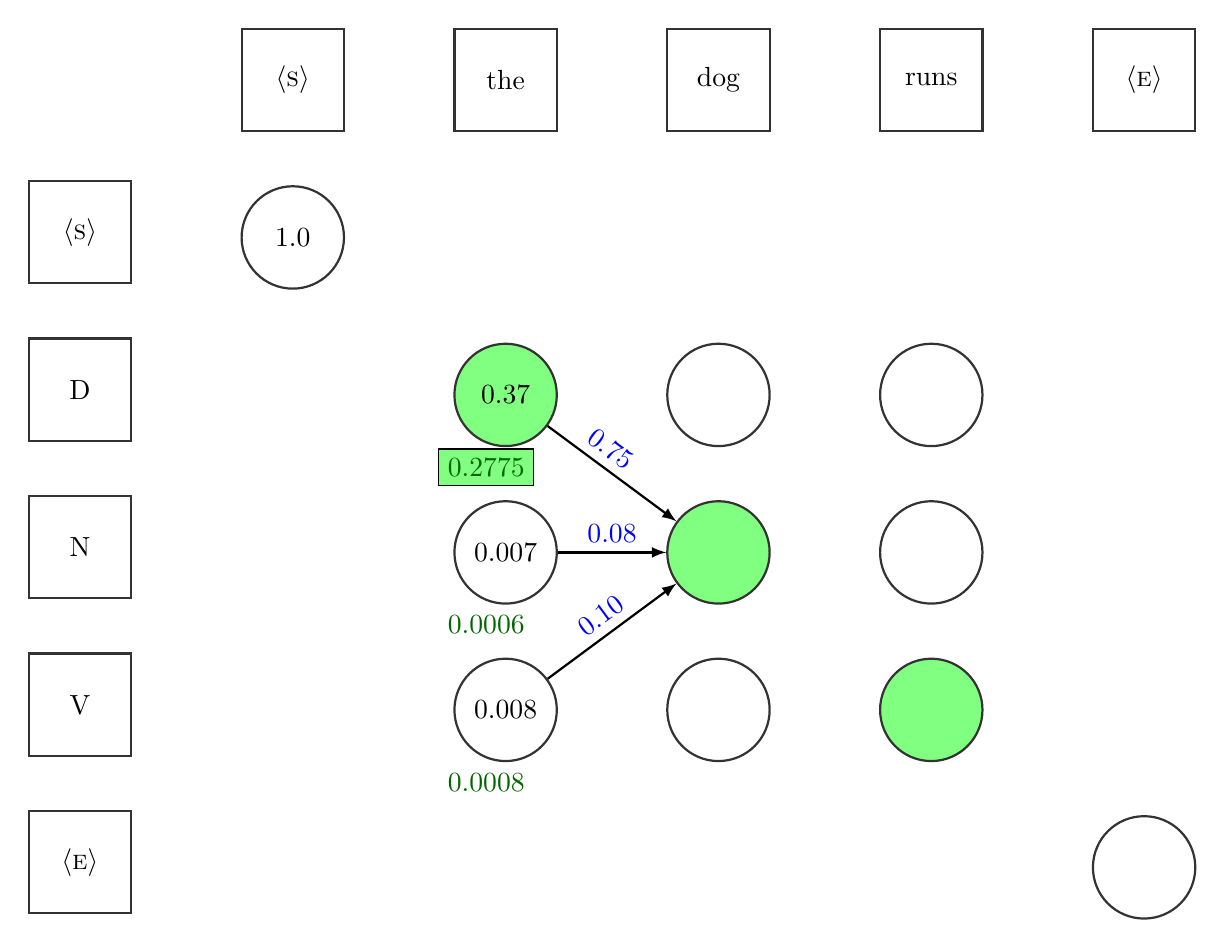
\begin{tikzpicture}
\tikzstyle{main}=[circle, thick, draw =black!80, node distance = 20mm, minimum size = 13mm]
\tikzstyle{rect}=[main, rectangle]
\tikzstyle{obsv}=[main, fill = black!10]
\tikzstyle{hidden}=[main, draw=white]
\tikzstyle{connect}=[-latex, thick]
\tikzstyle{box}=[rectangle, draw=black!100]

  
  \node[rect] (start) []                {\ngramstart};
  \node[rect] (D)     [below of =start] {D};
  \node[rect] (N)     [below of =D]     {N};
  \node[rect] (V)     [below of =N]     {V};
  \node[rect] (end)   [below of =V]     {\ngramend};

  \node[rect] (starttok) [right of =start,    xshift=20, yshift=55]   {\ngramstart};
  \node[rect] (the)      [right of =starttok, xshift=20]              {the};
  \node[rect] (dog)      [right of =the,      xshift=20]              {dog};
  \node[rect] (runs)     [right of =dog,      xshift=20]              {runs};
  \node[rect] (endtok)   [right of =runs,     xshift=20]              {\ngramend};

  \node[main] (startstart)  [below of =starttok]  {1.0};

  \node[hidden] (startthe)  [below of =the]       {};
  \node[main, fill=white!50!green] (Dthe)        [below of =startthe]  {0.37};
  \node[draw, fill=white!50!green] at ([shift={(75:-0.95)}]Dthe) {\color{black!60!green}0.2775};
  \node[main] (Nthe)        [below of =Dthe]      {0.007};
  \node[draw, draw=white] at ([shift={(75:-0.95)}]Nthe) {\color{black!60!green}0.0006};
  \node[main] (Vthe)        [below of =Nthe]      {0.008};
  \node[draw, draw=white] at ([shift={(75:-0.95)}]Vthe) {\color{black!60!green}0.0008};
  \node[hidden] (endthe)    [below of =Vthe]      {};

  \node[hidden] (startdog)  [below of =dog]       {};
  \node[main] (Ddog)        [below of =startdog]  {};
  \node[main, fill=white!50!green] (Ndog)        [below of =Ddog]      {};
  \node[main] (Vdog)        [below of =Ndog]      {};
  \node[hidden] (enddog)    [below of =Vdog]      {};

  \node[hidden] (startruns) [below of =runs]      {};
  \node[main] (Druns)       [below of =startruns] {};
  \node[main] (Nruns)       [below of =Druns]     {};
  \node[main, fill=white!50!green] (Vruns)       [below of =Nruns]     {};
  \node[hidden] (endruns)   [below of =Vruns]     {};

  \node[hidden] (startend)  [below of =endtok]    {};
  \node[hidden] (Dend)      [below of =startend]  {};
  \node[hidden] (Nend)      [below of =Dend]      {};
  \node[hidden] (Vend)      [below of =Nend]      {};
  \node[main]   (endend)    [below of =Vend]      {};


  
  \path (Dthe) edge [connect] node [pos=0.4, above, blue, sloped] {0.75} (Ndog);
  \path (Nthe) edge [connect] node [pos=0.5, above, blue, sloped] {0.08} (Ndog);
  \path (Vthe) edge [connect] node [pos=0.5, above, blue, sloped] {0.10} (Ndog);
  

\end{tikzpicture}
\caption{}
\end{figure} 




% \begin{align*}

% \end{align*}



\section{Tag Dictionary}

\begin{itemize}
  \item Mapping from words to potential tags
  \item Get from train, assume works on test
  \item Unseen words usually assumed to be any possible tag.  Could, instead, assume only open-class tags.
  \item Prune low-probability tags
\end{itemize}





\newsavebox{\startaltable}
\sbox{\startaltable}{
    \begin{tabular}{l l}
      \hline
      \multicolumn{2}{|c|}{{\cellcolor{gray!40}\ngramstart}} \tabularnewline
      \hline
      \ngramstart & 1.0
    \end{tabular}
}

\newsavebox{\Daltable}
\sbox{\Daltable}{
    \begin{tabular}{l l}
      \hline
      \multicolumn{2}{|c|}{{\cellcolor{gray!40}D}} \tabularnewline
      \hline
      the & 0.47 \tabularnewline
      a   & 0.12 \tabularnewline
      $*$   & 0.06
    \end{tabular}
}

\newsavebox{\Naltable}
\sbox{\Naltable}{
    \begin{tabular}{l l}
      \hline
      \multicolumn{2}{|c|}{{\cellcolor{gray!40}N}} \tabularnewline
      \hline
      man & 0.24 \tabularnewline
      dog & 0.29 \tabularnewline
      cat & 0.12 \tabularnewline
      $*$   & 0.06
    \end{tabular}
}

\newsavebox{\Valtable}
\sbox{\Valtable}{
    \begin{tabular}{l l}
      \hline
      \multicolumn{2}{|c|}{{\cellcolor{gray!40}V}} \tabularnewline
      \hline
      walks  & 0.33 \tabularnewline
      runs   & 0.13 \tabularnewline
      saw    & 0.13 \tabularnewline
      $*$      & 0.07
    \end{tabular}
}

\newsavebox{\ngramendaltable}
\sbox{\ngramendaltable}{
    \begin{tabular}{l l}
      \hline
      \multicolumn{2}{|c|}{{\cellcolor{gray!40}\ngramend}} \tabularnewline
      \hline
      \ngramend & 1.0
    \end{tabular}
}


\begin{figure}[h]
\centering
\begin{tikzpicture}
\tikzstyle{main}=[rectangle, thick, draw =black!80, node distance = 40mm]
\tikzstyle{obsv}=[main, fill = black!10]
\tikzstyle{hidden}=[node distance = 16mm]
\tikzstyle{connect}=[-latex, thick]
\tikzstyle{box}=[rectangle, draw=black!100]

  \node[main] (start) []                         {\usebox{\startaltable}};
  \node[main] (D)     [right of =start]          {\usebox{\Daltable}};
  \node[main] (N)     [right of =D, yshift= 90]  {\usebox{\Naltable}};
  \node[main] (V)     [right of =D, xshift=60, yshift=-90]  {\usebox{\Valtable}};
  \node[main] (end)   [right of =D, xshift=170]   {\usebox{\ngramendaltable}};


  \path (start) edge [connect] node [pos=0.5, above, blue, sloped] {0.78} (D);
  \path (start) edge [connect, bend left=25] node [pos=0.5, above, blue, sloped] {0.11} (N);
  \path (start) edge [connect, bend right=25] node [pos=0.5, below, blue, sloped] {0.11} (V);
  
  \path (D) edge [in=98,out=83,loop] node [pos=0.5, above, blue, sloped] {0.08} (D);
  \path (D) edge [connect, bend left=15] node [pos=0.5, above, blue, sloped] {0.75} (N);
  \path (D) edge [connect, bend right=15] node [pos=0.5, below, blue, sloped] {0.08} (V);
  \path (D) edge [connect, bend left=10] node [pos=0.75, above, blue, sloped] {0.08} (end);

  \path (N) edge [connect, bend left=15, red] node [pos=0.5, above, blue, sloped] {0.08} (D);
  \path (N) edge [in=98,out=83,loop] node [pos=0.5, above, blue, sloped] {0.08} (N);
  \path (N) edge [connect, bend left=15] node [pos=0.5, below, blue, sloped] {0.58} (V);
  \path (N) edge [connect] node [pos=0.5, above, blue, sloped] {0.25} (end);

  \path (V) edge [connect, bend right=15, red] node [pos=0.5, below, blue, sloped] {0.30} (D);
  \path (V) edge [connect, bend left=15, red] node [pos=0.5, below, blue, sloped] {0.10} (N);
  \path (V) edge [in=-98,out=-83,loop] node [pos=0.5, below, blue, sloped] {0.10} (V);
  \path (V) edge [connect] node [pos=0.5, below, blue, sloped] {0.50} (end);
  

\end{tikzpicture}
\caption{Finite state machine.  Missing arrows are assumed to be zero probabilities.  With smoothing, there is an arrow in \textit{both directions} between every pair of tags.}
\end{figure} 







\end{document}

